\documentclass[9pt]{beamer}

\usetheme[progressbar=frametitle]{metropolis}
\usepackage{appendixnumberbeamer}

\usepackage{booktabs}
\usepackage[scale=2]{ccicons}
\usepackage{subfigure}
\usepackage{pgfplots}
\usepgfplotslibrary{dateplot}

\usepackage{xspace}
\newcommand{\themename}{\textbf{\textsc{metropolis}}\xspace}

\usepackage{caption}
%\usepackage{gensymb}
\usepackage{ulem}
%\usepackage{subcaption}
\usepackage[french]{babel}
\usepackage{csquotes}
\usepackage[backend=biber,style=authoryear,citestyle=authoryear]{biblatex}
\usepackage{tikz}
\usetikzlibrary{positioning}

\DeclareCaptionLabelFormat{underlcap}{\uline{#1 #2}}
\DeclareCaptionLabelSeparator{underlcap}{~}
\DeclareCaptionTextFormat{underlcap}{\expandafter\uline\expandafter{\expandafter#1}}

\captionsetup[figure]{%
   labelformat=underlcap,labelseparator=underlcap,textformat=underlcap}
   
\newcommand\Wider[2][3em]{%
\makebox[\linewidth][c]{%
  \begin{minipage}{\dimexpr\textwidth+#1\relax}
  \raggedright#2
  \end{minipage}%
  }%
}

\makeatletter
\setlength{\metropolis@progressinheadfoot@linewidth}{1.7pt}
\setlength{\metropolis@titleseparator@linewidth}{1.7pt}
\setlength{\metropolis@progressonsectionpage@linewidth}{1.7pt}

\definecolor{alizarin}{rgb}{0.1, 0.26, 0.82}
\definecolor{bazaar}{rgb}{0.63, 0.63, 0.8}

\setbeamercolor{progress bar}{fg=alizarin,bg=bazaar}

\AtBeginSection[]{
  \begin{frame}
  \vfill
  \centering
  \begin{beamercolorbox}[sep=8pt,center,shadow=true,rounded=true]{title}
    \usebeamerfont{title}\insertsectionhead\par%
  \end{beamercolorbox}
  \vfill
  \end{frame}
}

\addbibresource{/Applications/ZoteroBibs/Library.bib}

\begin{document}

\title{Concours de l'école doctorale des Sciences de l'Environnement}
\subtitle{Sujet: Étude de la morphologie des nuages de couche limite et de leur rôle dans la sensibilité climatique \\ ~\\
\textit{Proposé par Florent Brient et Sandrine Bony}}
\date{\today}
\author{\textbf{Félix Langot}}
\institute{\includegraphics[width=3.6cm]{/Users/felixlangot/Pictures/Icons/university-of-bristol-2.png}\hfill
\includegraphics[width=3.9cm]{Figures/LMDSorbonne.png}\hfill\includegraphics[width=2.7cm]{/Users/felixlangot/Pictures/Icons/logo-uvsq-2020-actu.png}}
%\titlegraphic{
\includegraphics[height=1.5cm]{Figures/logo.png}}
{\usebackgroundtemplate{\tikz\node[opacity=0.1, anchor=center]{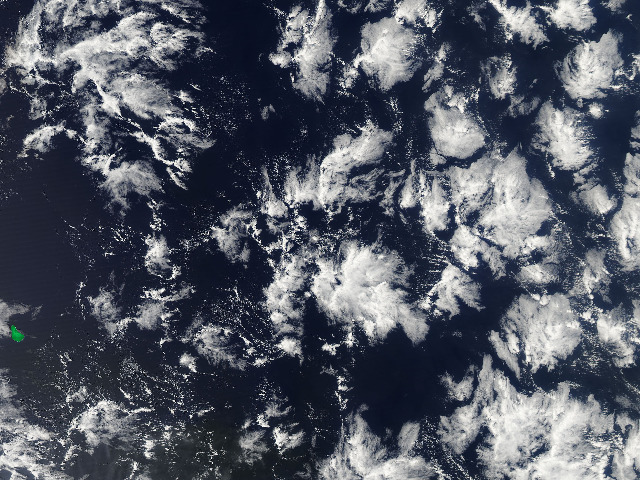
\includegraphics[width=20cm]{Figures/Flowers.jpeg}};}
% {\usebackgroundtemplate{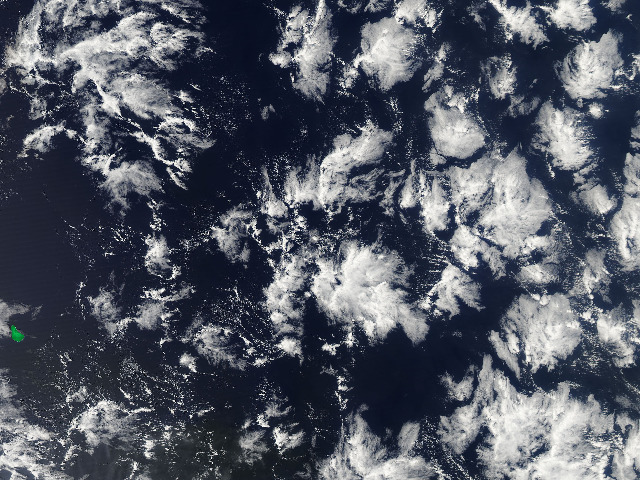
\includegraphics{Figures/Flowers.jpeg}}
\begin{frame}[plain,noframenumbering]
  \maketitle
\end{frame}
}

% \begin{frame}
%   \maketitle
%   \begin{tikzpicture}[overlay, remember picture]
%   \node[above right=1cm and .8cm of current page.south west] {
\includegraphics[width=2cm]{Figures/logo.png}};
%   \node[above =1cm of current page.south] {
\includegraphics[width=2cm]{Figures/logo.png}};
%   \node[above left=1cm and .8cm of current page.south east] {
\includegraphics[width=2cm]{Figures/logo.png}};
%   \end{tikzpicture}
%   \end{frame}
%   \end{document}

\section*{Présentation du cursus}
\begin{frame}{\secname}
\Wider{
\textbf{Baccalauréat S (2016):} 
  \begin{itemize}
      \item mention TB, mention européenne, spécialité mathématiques.
      \item 17.5 de moyenne générale dont 19/20 en mathématiques et 17/20 en physique
  \end{itemize} 
\vspace{0.35cm}
\textbf{MSci Physics with Astrophysics, Bristol, UK (2020):} ~~~~~~~~~~\includegraphics[width=2cm]{/Users/felixlangot/Pictures/Icons/university-of-bristol-2.png} 
  \begin{itemize}
      \item Obtention du master avec 'Upper second class honours' (mention B)
      \item 'Commendation' pour le projet final de master (note > 16)
      \item Passage de plusieurs unités avec des notes '1st class' (mention TB) y compris dans l'UE \textit{Geophysical Fluid Dynamics}
  \end{itemize}
  \vspace{0.35cm}
  \begin{tikzpicture}[overlay, remember picture]
    \node[above left=1.7cm and .8cm of current page.south east] {\includegraphics[width=1.7cm]{/Users/felixlangot/Pictures/Icons/logo-uvsq-2020-actu.png}};
    \node[above left=0.8cm and .8cm of current page.south east] {
\includegraphics[width=2.5cm]{Figures/LMDSorbonne.png}};
  \end{tikzpicture}
\textbf{Master Étude des Climats de la Terre, Paris, FR (2021):}
  \begin{itemize}
      \item Moyenne du premier semestre de 15.4/20
      \item 18/20 de moyenne dans les U.E. de modélisation
  \end{itemize}
}
\end{frame}

\section*{Expériences de recherche}
\begin{frame}{\secname}
\Wider{ 
  \vspace{-3.5cm} 
  \begin{columns}
  \column{0.6\textwidth}
    \textbf{~~~~~~~MSci Project} (avec Dr. B. Maughan): 
    \begin{itemize}
      \item Estimation de la vitesse d'expansion de l'Univers
      \item Calcul des distances, analyse de données, travail théorique pour interprétation
    \end{itemize}
  \column{0.5\textwidth}
  \vspace{0.1cm}
    \begin{figure}[hbtp]
      \centering
      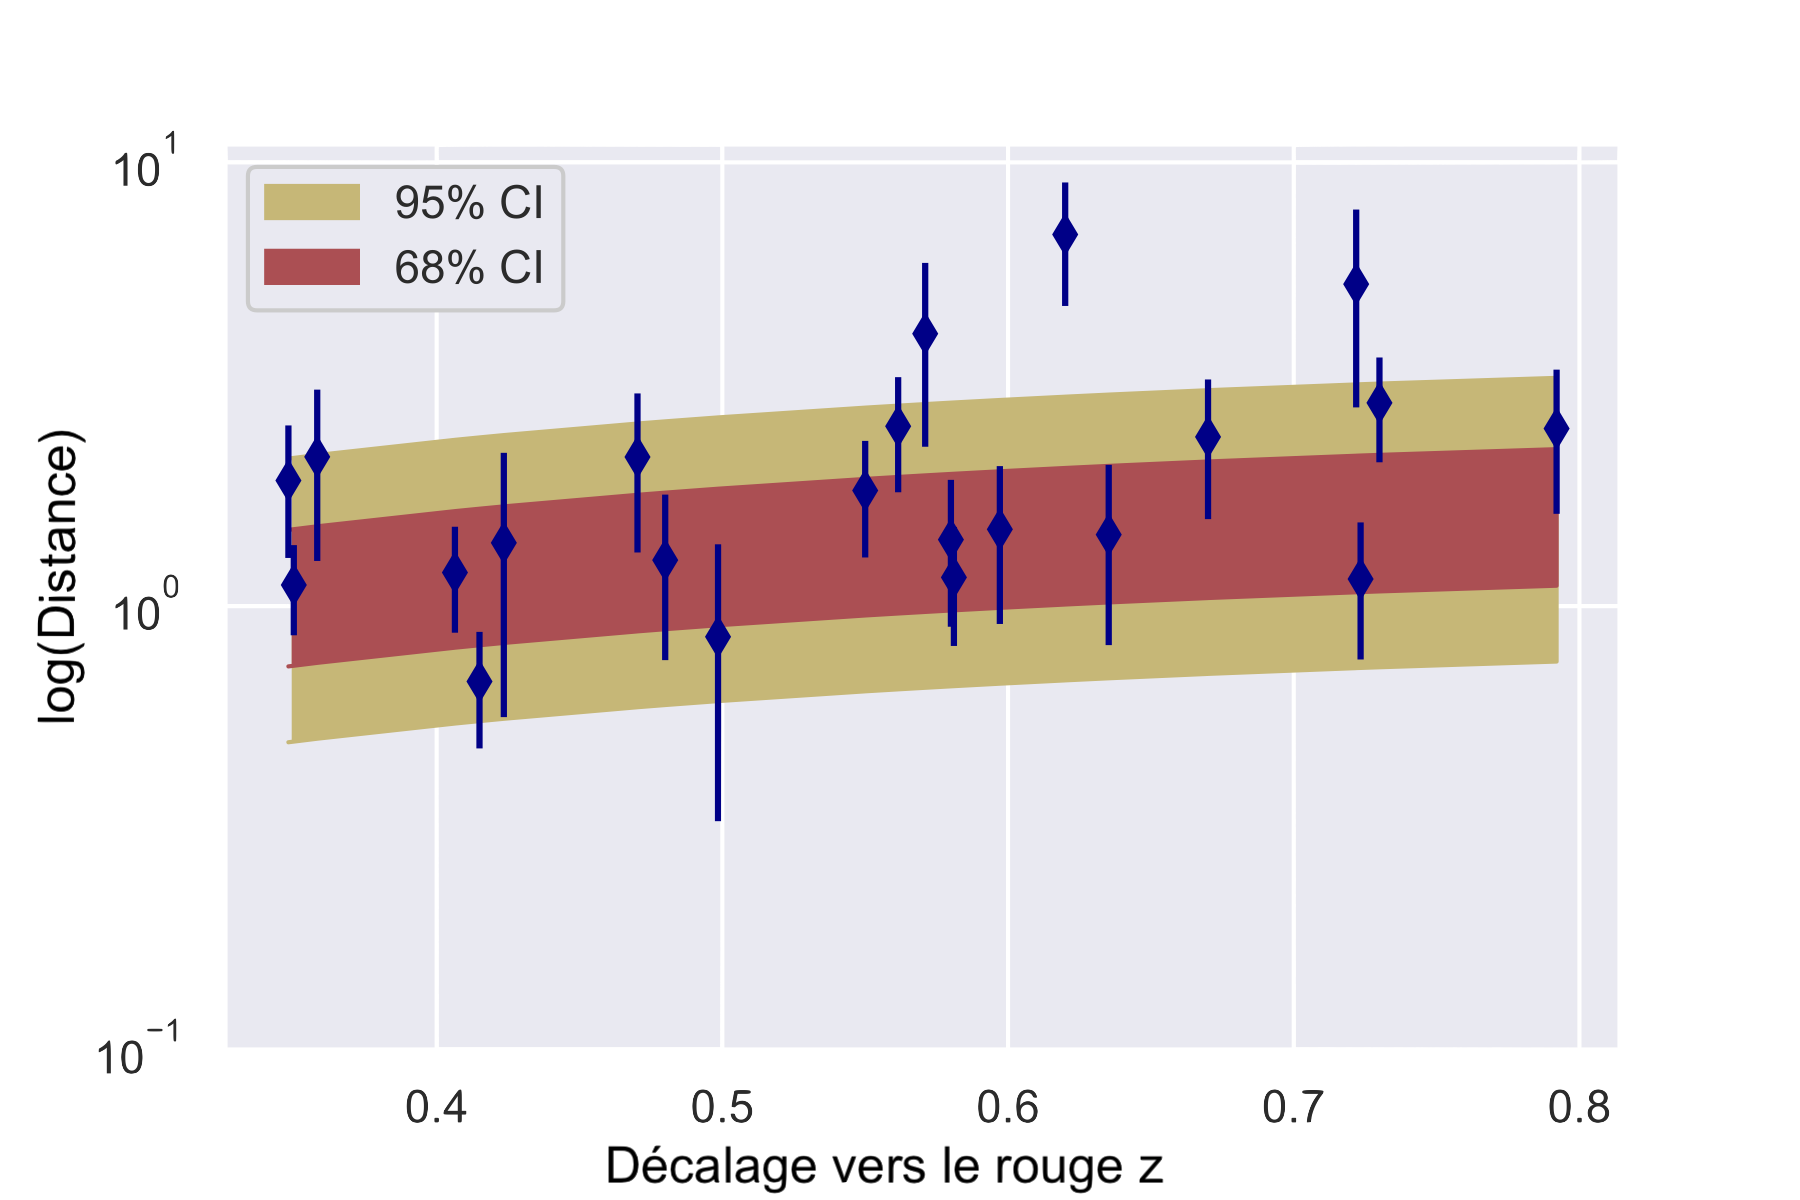
\includegraphics[width=6cm]{Figures/Logs.png}
    \end{figure}
\end{columns}
\pause
\vspace{-0.5cm}
\textbf{Stage de M2} (avec Dr. C. Risi):
\begin{itemize}
  \item Stage au LMD: Impact de l'organisation de la convection profonde sur l'humidité de la troposphère
\end{itemize}
}
\begin{tikzpicture}[overlay, remember picture]
  \node[above =0cm of current page.south]
  {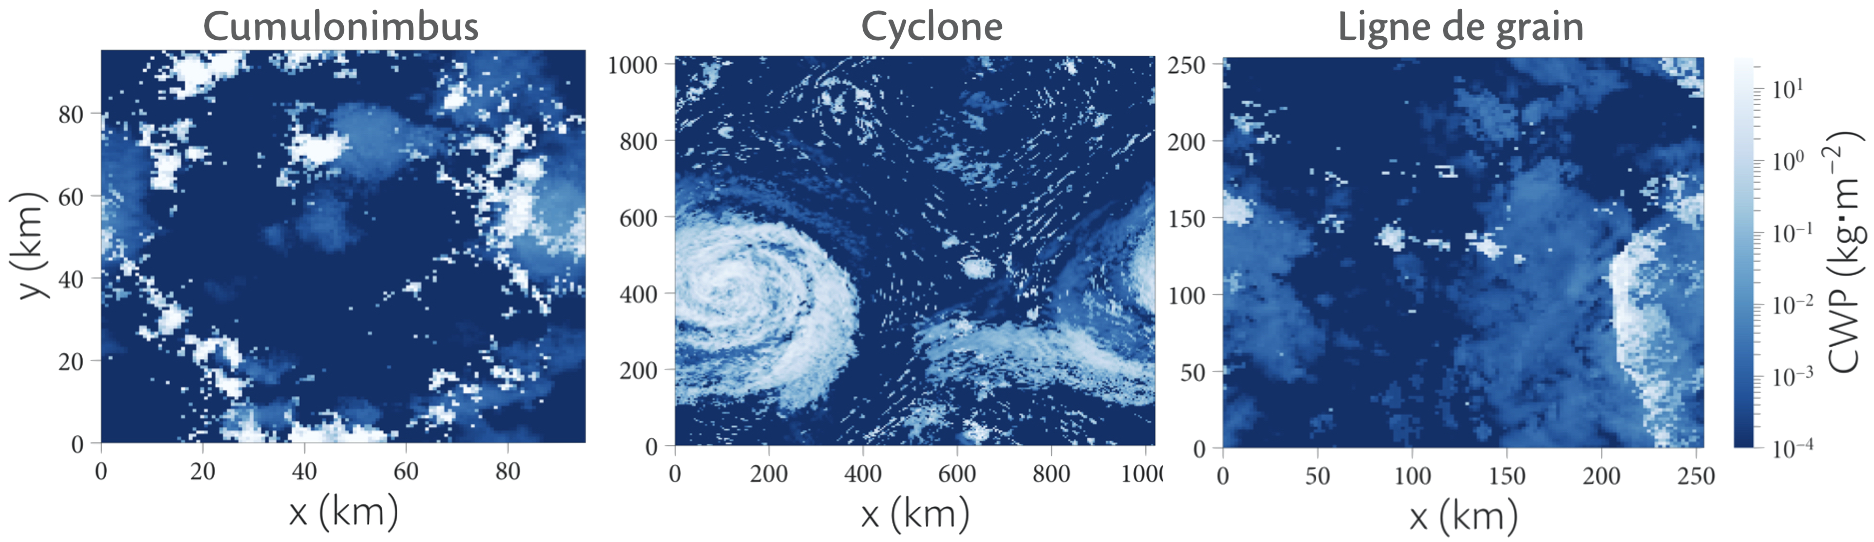
\includegraphics[width=12cm]{Figures/VisAssemble2.png}};
  \end{tikzpicture}
\end{frame}

\begin{frame}{\secname}
\vspace{-0.3cm}
\Wider{
\begin{columns}
  \column{0.52\textwidth}
  \begin{itemize}
    \item Construction d'un modèle simple 
    \item Comparaison avec simulations sur cloud-resolving model (CRM)
    \item Décomposition et quantification des facteurs influençant l'humidité
  \end{itemize}
  \column{0.52\textwidth}
  \vspace{-0cm}
  \begin{figure}[hbtp]
    \centering
    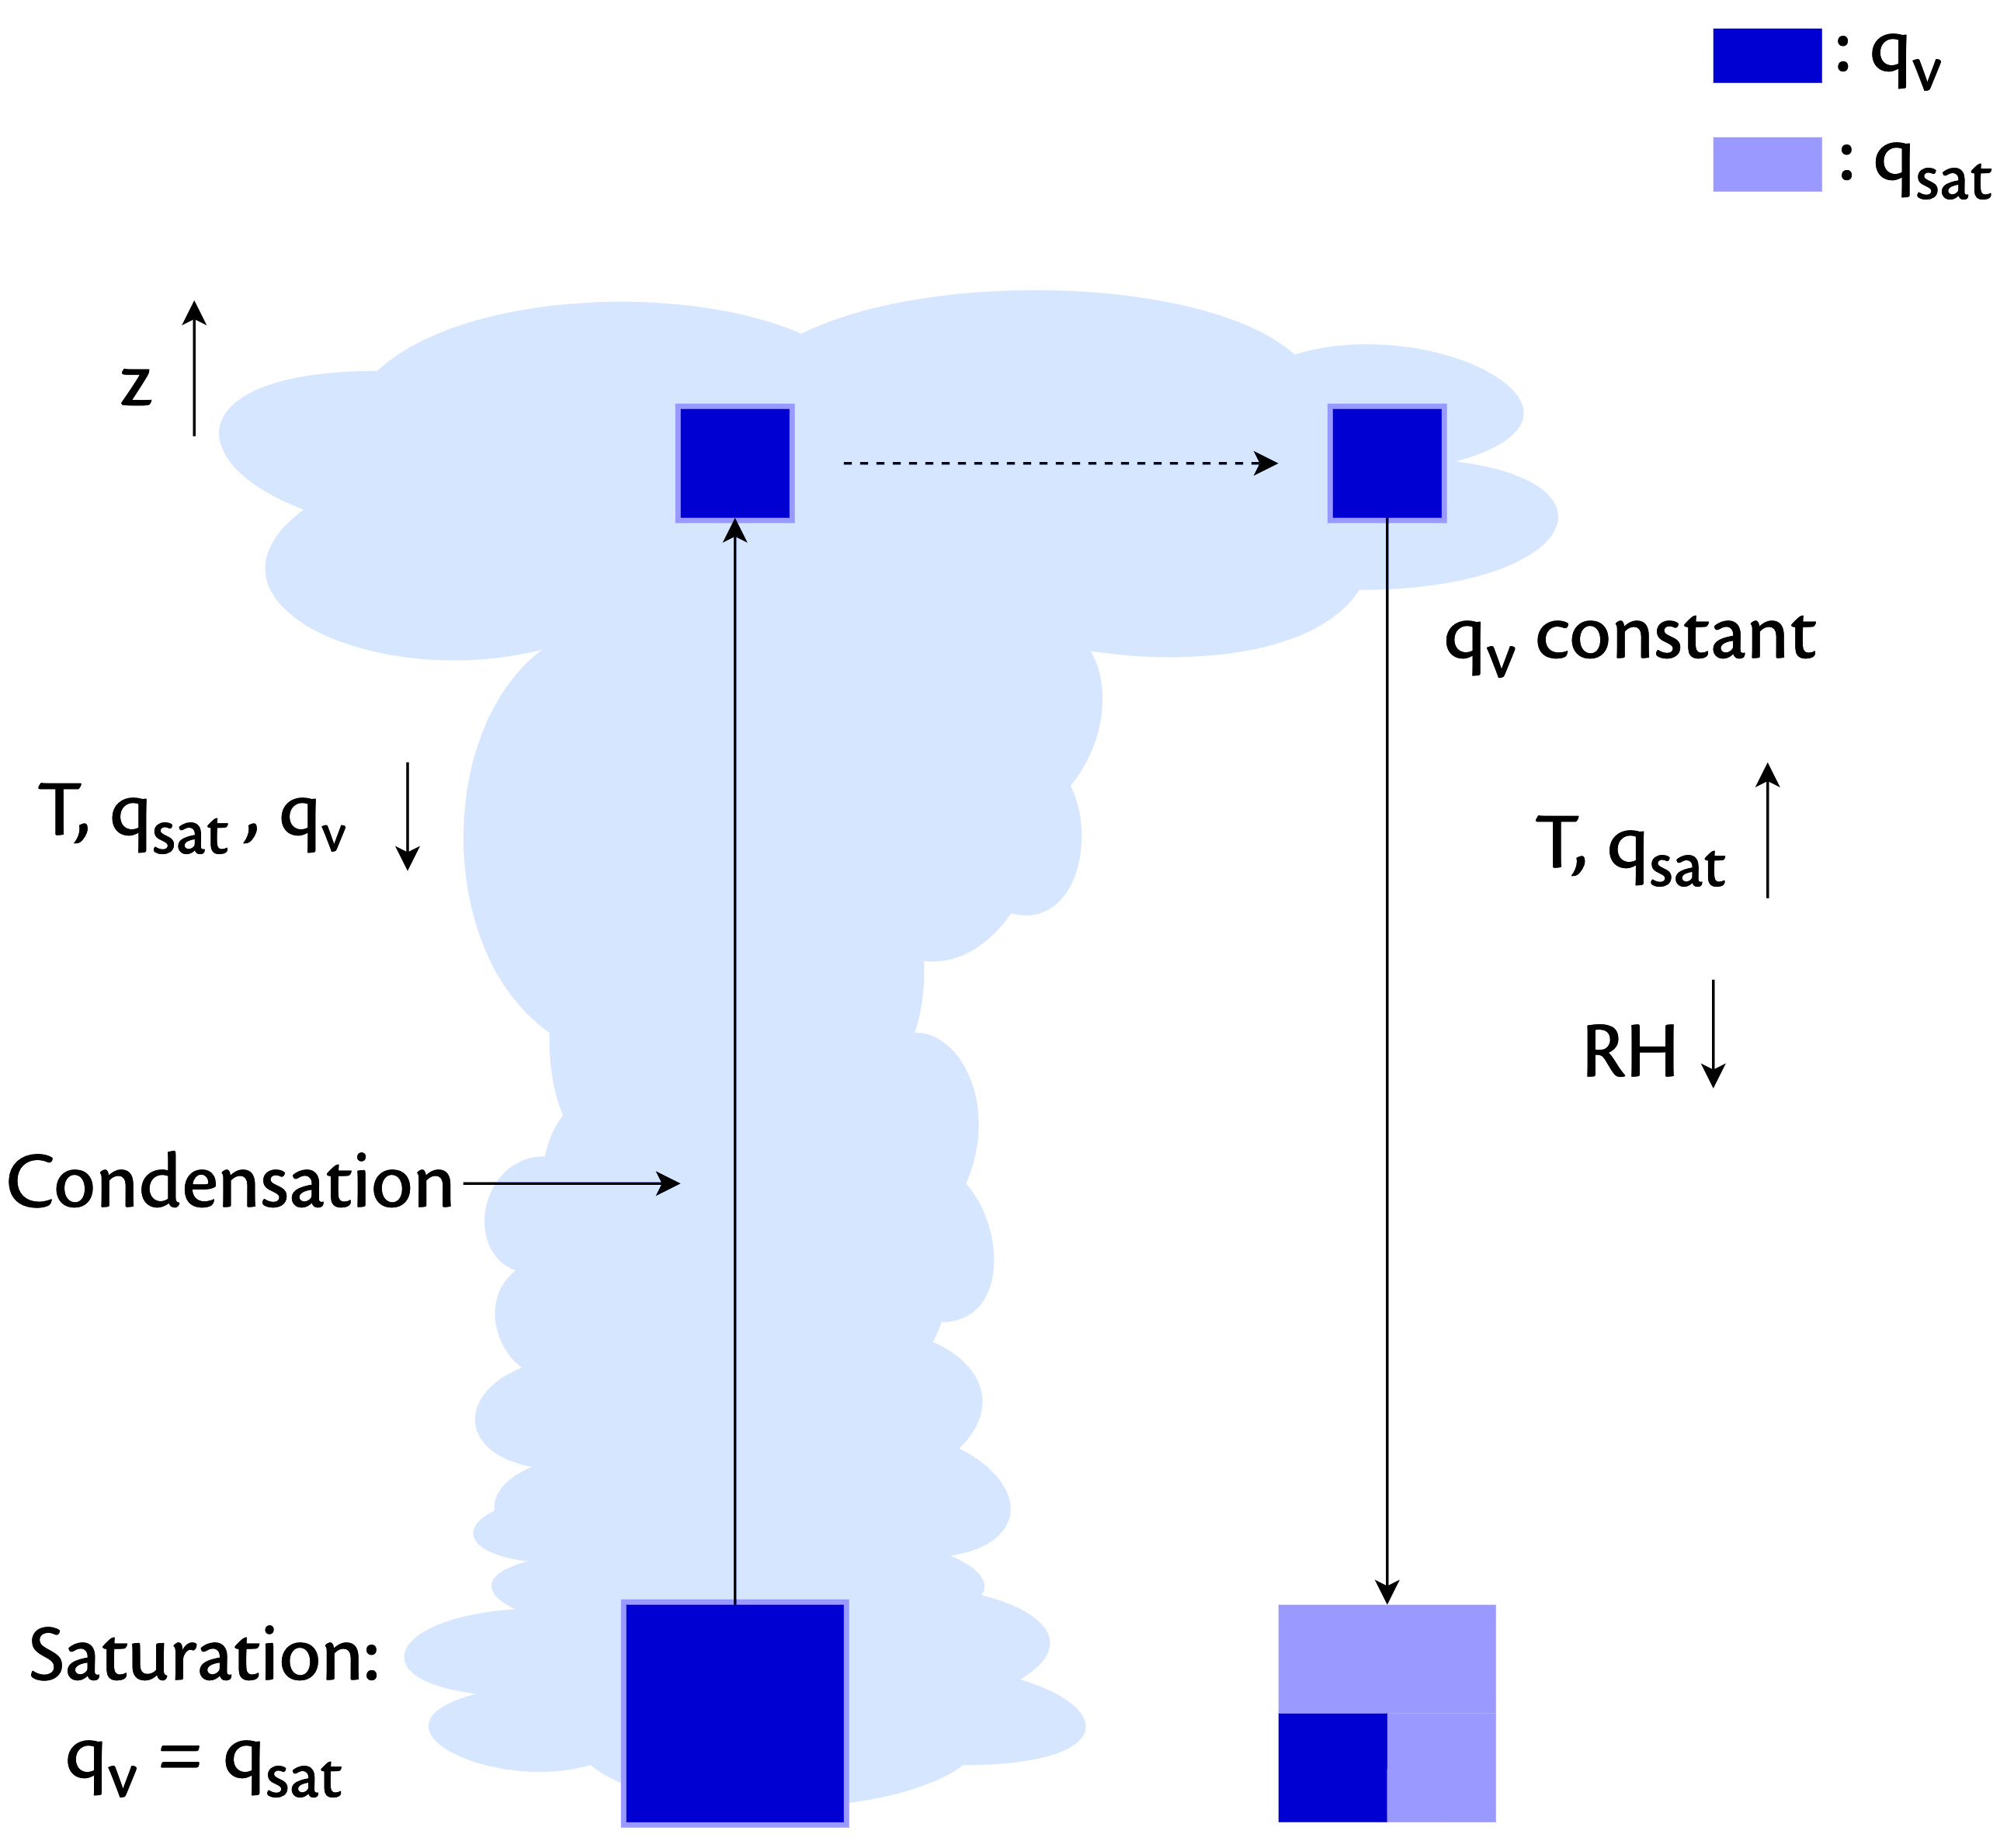
\includegraphics[width=4.2cm]{Figures/advec-condens.png}
  \end{figure}
\end{columns}
\vspace{-0cm}
\begin{figure}
  \subfigure{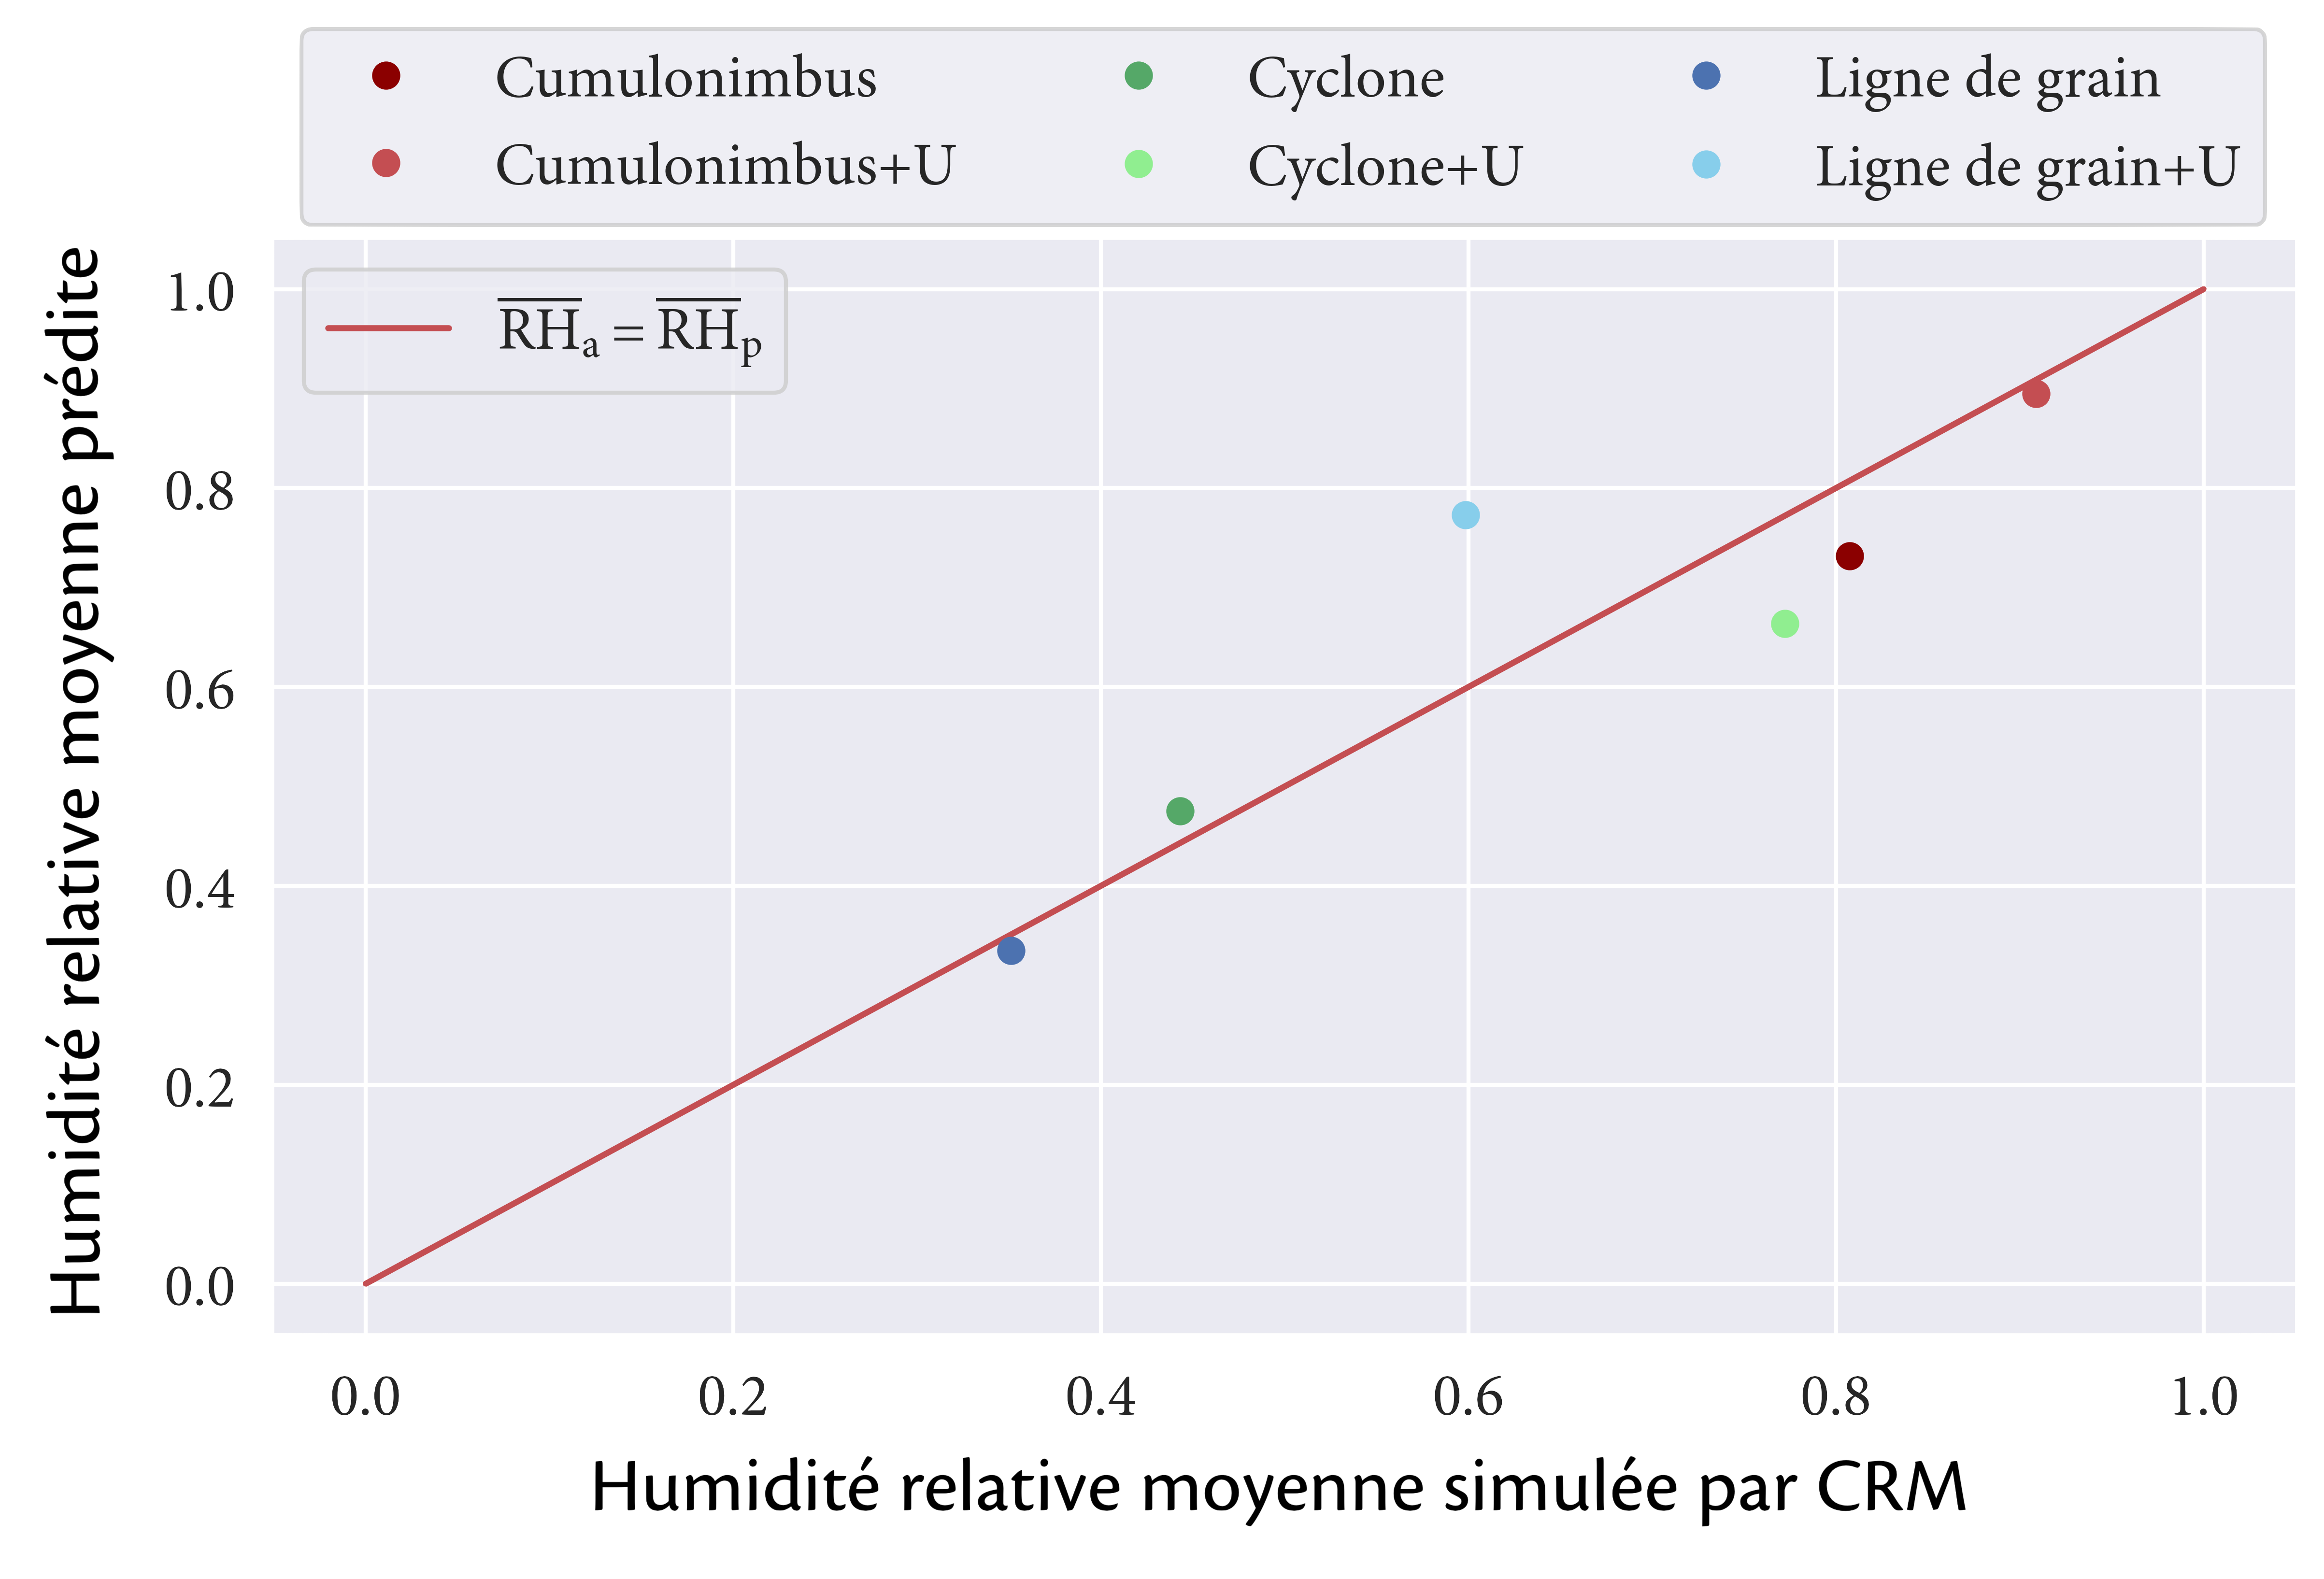
\includegraphics[width=5.3cm]{/Users/felixlangot/Stage/GitRepos/Codes/Figs/meanRHpvsRHa.png}}
  \hfill \hspace{-1cm}
  \subfigure{\raggedright\includegraphics[width=5.3cm]{/Users/felixlangot/Stage/GitRepos/Codes/Figs/OrgComps.png}}
\end{figure}

}
\end{frame}

\section*{Projet}
\begin{frame}{\secname}
% \begin{tikzpicture}[overlay, remember picture]
%   \node[below =1cm of current page.north]
%   {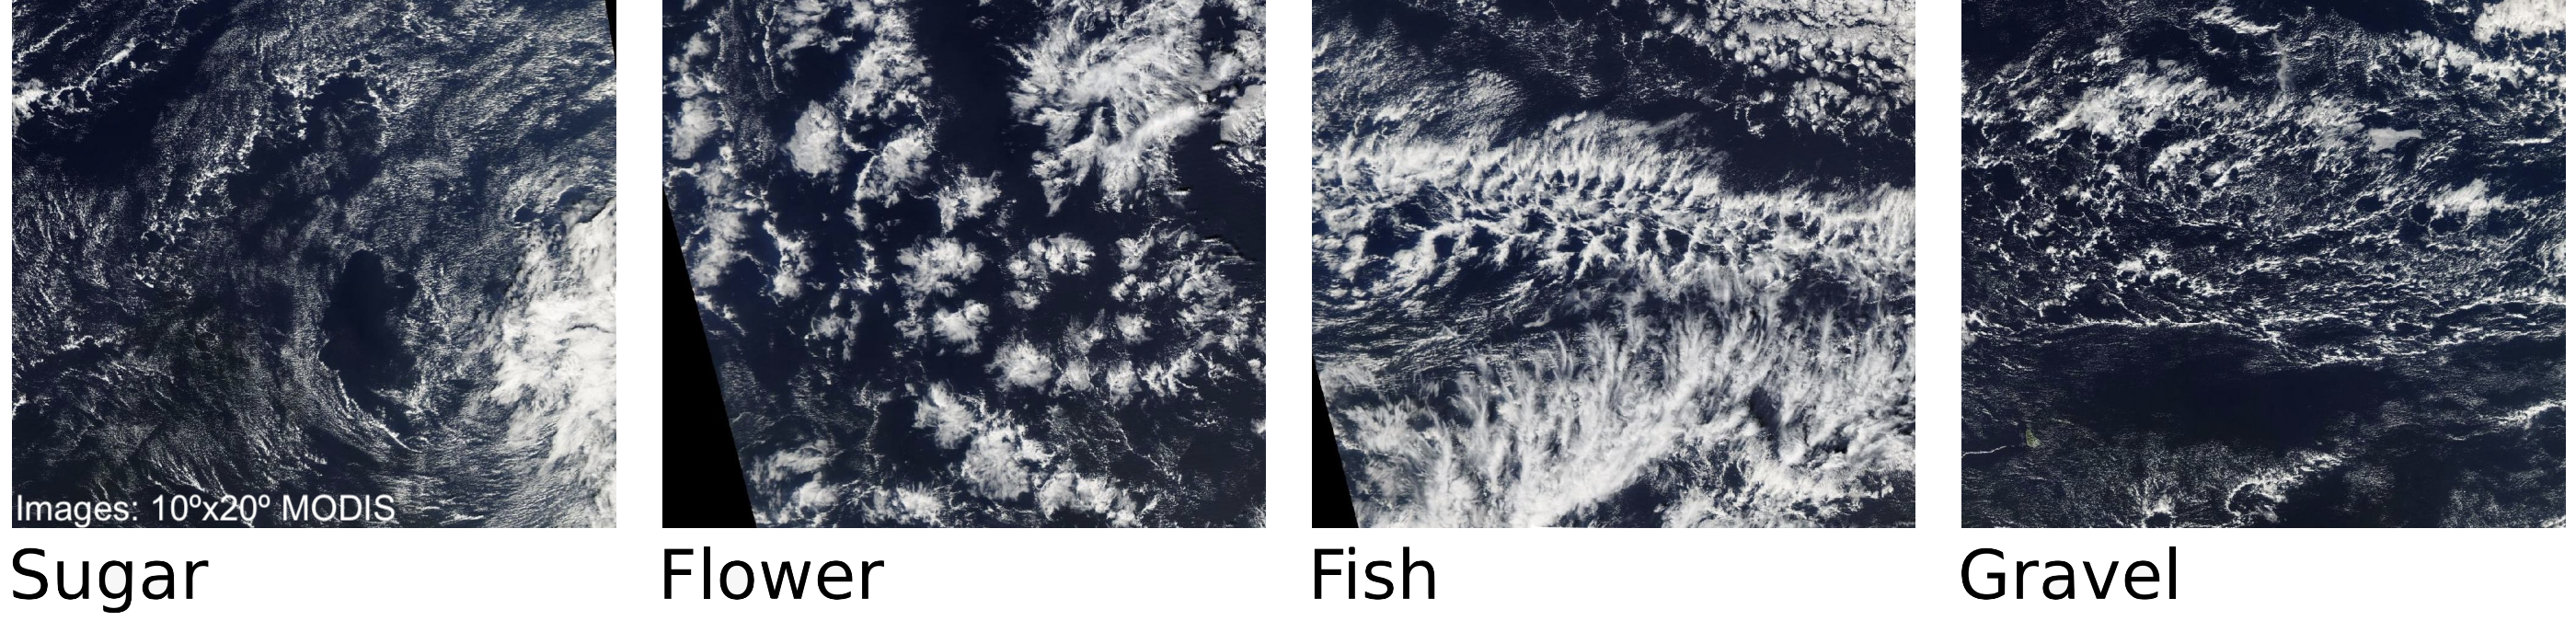
\includegraphics[width=11.2cm]{Figures/SugGravFishFlo.png}};
%   \end{tikzpicture}
\Wider{
  % \vspace{2.7cm}
\textbf{Contexte:}
\begin{itemize}
  \item Projections climatiques incertaines principalement à cause des nuages de couche limite
\end{itemize}
\pause
\begin{figure}
  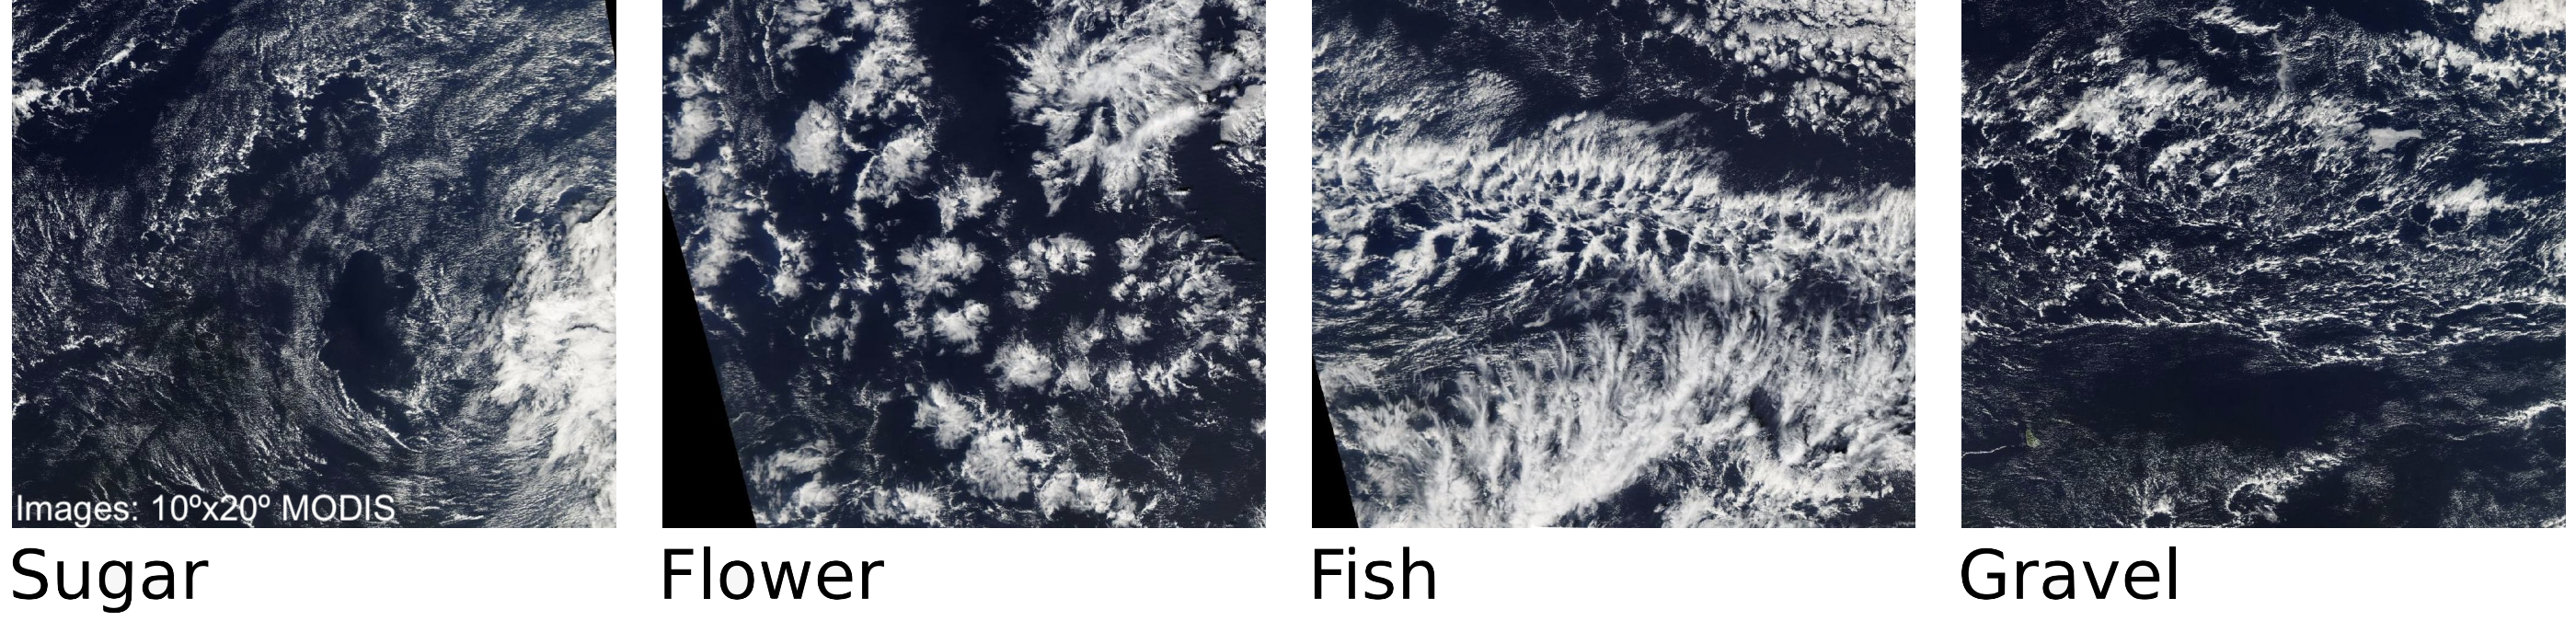
\includegraphics[width=11.2cm]{Figures/SugGravFishFlo.png}
\end{figure}
\textbf{But:}
\begin{itemize}
  \item Comprendre le rôle de l'organisation de ces nuages sur leur rétroaction climatique
\end{itemize}
\pause
\textbf{Étapes:}
\begin{itemize}
  \item Catégoriser les morphologies (IA)
  \item Analyser les relations entre morphologies et environnement
  \item Étendre l'analyse avec des modèles de haute résolution
\end{itemize}
}
\end{frame}

{\usebackgroundtemplate{\tikz\node[opacity=0.2]{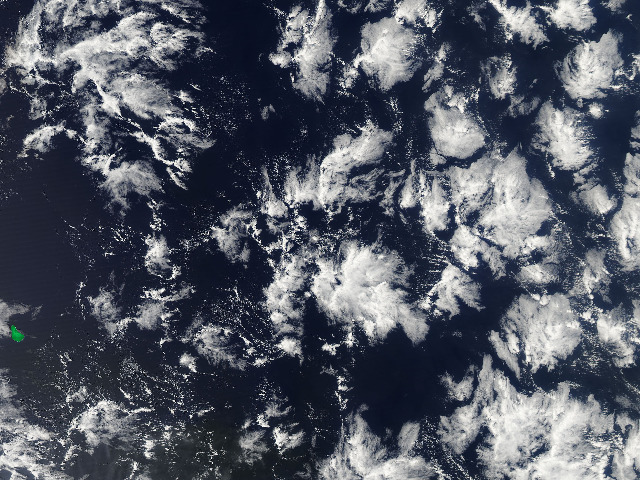
\includegraphics[width=\paperwidth]{Figures/Flowers.jpeg}};}
\begin{frame}
  \centering
  \Large 
  \textcolor{black}{Merci pour votre attention!}
\end{frame}
}

\begin{frame}
  \includegraphics[width=\textwidth]{Figures/SchémaBilan.png}
\end{frame}

\end{document}
